\subsection{Specular}

\begin{frame}{Specular Reflection - Introduction}
  \begin{columns}
    \begin{column}{0.6\textwidth}
      \begin{conceptbox}{Shiny Surfaces}
        \footnotesize
        \textbf{Examples:}

        Mirrors, metals, plastic

        \vspace{0.3cm}
        \textbf{Characteristics:}
        \begin{itemize}
          \item View-dependent brightness
          \item Creates highlights
          \item Follows law of reflection
          \item Intensity depends on viewing angle
        \end{itemize}
      \end{conceptbox}
    \end{column}
    \begin{column}{0.4\textwidth}
      \begin{center}
        \begin{tikzpicture}[scale=0.8]
          \draw[ObjectColor, very thick] (-2,0) -- (2,0);
          \fill[ObjectColor] (0,0) circle (3pt);

          \draw[->, PrimaryColor, thick] (0,0) -- (0,1.5);
          % \node[right] at (0.1,0.75) {\footnotesize $\mathbf{N}$};

          \draw[->, lightray, thick] (0,0) -- (-0.6,0.6) node[left, black] {\footnotesize $\mathbf{L}$};

          \draw[->, AccentColor, thick] (0,0) -- (1.2,1.2) node[above, anchor=west, black] {\scriptsize $\mathbf{V}_1$ (bright)};
          \draw[->, AccentColor, thick] (0,0) -- (0.8,1.5) node[above, anchor=west, black] {\scriptsize $\mathbf{V}_2$ (dim)};
          \draw[->, AccentColor, thick] (0,0) -- (-0.8,1.5) node[above, black] {\scriptsize $\mathbf{V}_3$ (dark)};
          \draw[->, reflectray, thick] (0,0) -- (0.6,0.6) node[right] {\footnotesize $\mathbf{R}$};
        \end{tikzpicture}

        \only<2->{
          \vspace{0.3cm}
          \begin{figure}
            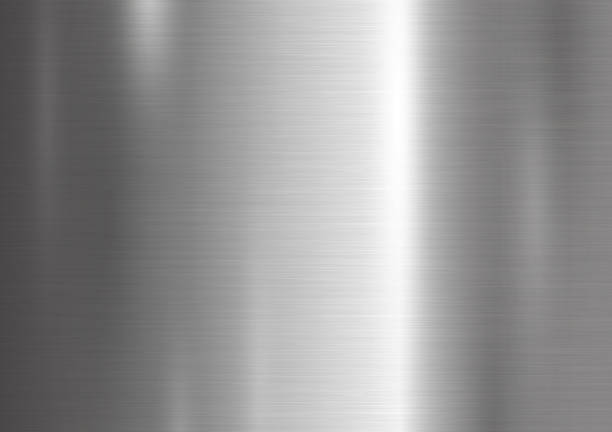
\includegraphics[width=0.6\linewidth]{images/metal.jpg}
            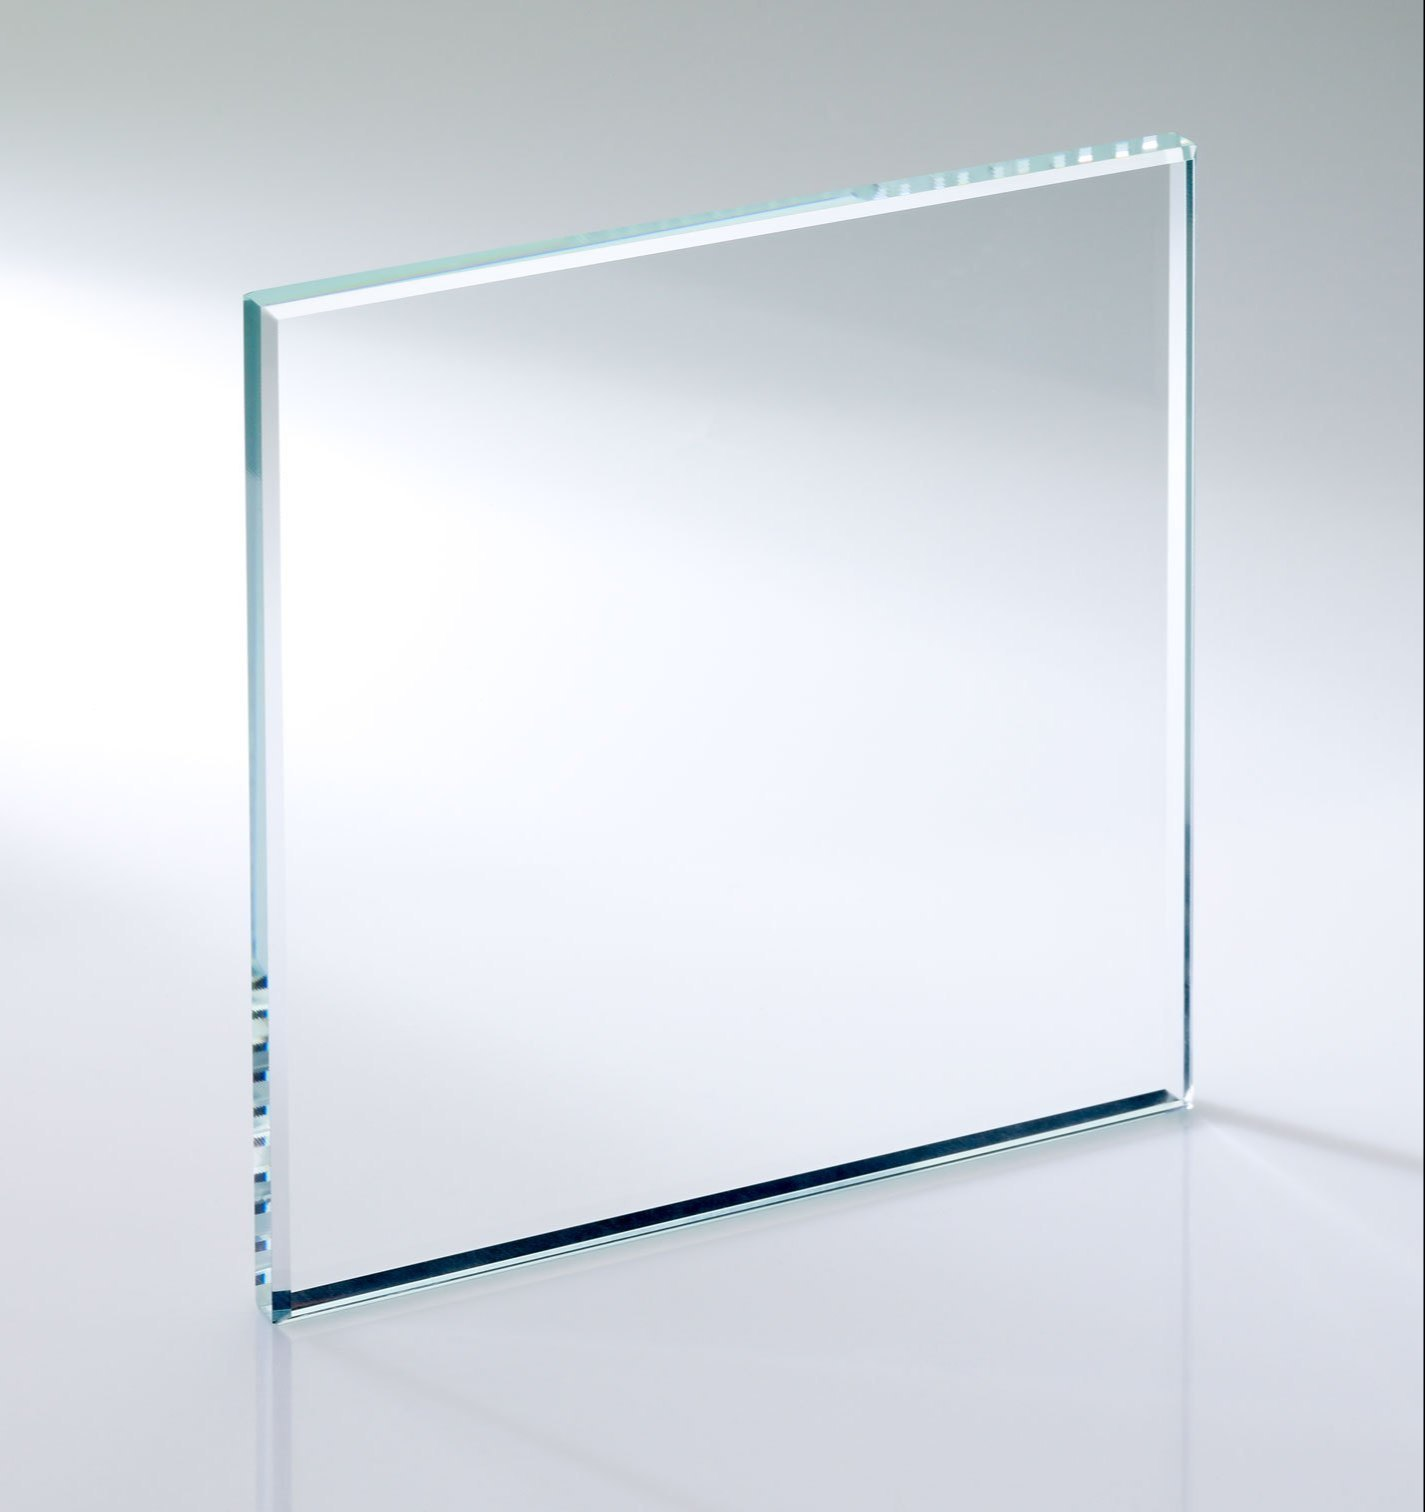
\includegraphics[width=0.6\linewidth]{images/glass.jpg}
            \caption*{\scriptsize Examples of diffuse surfaces: metal and glass}
          \end{figure}
        }
      \end{center}
    \end{column}
  \end{columns}
\end{frame}

\begin{frame}{Perfect Reflection Theory}
  \begin{columns}
    \begin{column}{0.6\textwidth}
      \begin{mathbox}{Law of Reflection}
        \footnotesize
        \textbf{Physical principle:} Angle of incidence equals angle of reflection

        \vspace{0.3cm}
        \textbf{Vector formulation:}
        \begin{align*}
          \mathbf{R} = 2(\mathbf{N} \cdot \mathbf{L})\mathbf{N} - \mathbf{L}
        \end{align*}

        where:
        \begin{itemize}
          \item $\mathbf{R}$ = reflection direction
          \item $\mathbf{N}$ = surface normal
          \item $\mathbf{L}$ = direction to light source
        \end{itemize}
        \only<2->{
          \vspace{0.3cm}
          \textbf{Derivation:} Decompose $\mathbf{L}$ into normal and tangential components
          \begin{align*}
            \mathbf{L}_{\parallel} &= (\mathbf{N} \cdot \mathbf{L})\mathbf{N} \\
            \mathbf{L}_{\perp} &= \mathbf{L} - \mathbf{L}_{\parallel} \\
            \mathbf{R} &= \mathbf{L}_{\parallel} - \mathbf{L}_{\perp}  =  2\mathbf{L}_{\parallel} - \mathbf{L}
          \end{align*}
        }
      \end{mathbox}
    \end{column}
    \begin{column}{0.4\textwidth}
      \begin{tikzpicture}[scale=0.8]
        \draw[ObjectColor, very thick] (-2,0) -- (2,0);

        \draw[->, PrimaryColor, thick] (0,0) -- (0,2) node[above] {\footnotesize $\mathbf{N}$};

        \draw[->, lightray, thick] (0,0) -- (-1.5,1.5) node[left] {\footnotesize $\mathbf{L}$};

        \draw[->, reflectray, thick] (0,0) -- (1.5,1.5) node[right] {\footnotesize $\mathbf{R}$};

        \draw[-] (0,1) arc [start angle=90, end angle=135, radius=1cm] node[midway, below] {\footnotesize $\theta_i$};
        \draw[-] (0,1) arc [start angle=90, end angle=45, radius=1cm] node[midway, below] {\footnotesize $\theta_r$};

        \only<2->{
          \draw[->, blue, thick] (0,0) -- (0,1.5) node[right] {\footnotesize $\mathbf{L}_{\parallel}$};
          \draw[->, red, thick] (0,0) -- (-1.5,0) node[below] {$\mathbf{L}_{\perp}$};
          \draw[->, orange, thick] (0,0) -- (1.5,0) node[below] {$-\mathbf{L}_{\perp}$};
        }
        \node[below] at (0,-1) {\footnotesize $\theta_i = \theta_r$};
        \fill[ObjectColor] (0,0) circle (3pt);
      \end{tikzpicture}
    \end{column}
  \end{columns}
\end{frame}

\begin{frame}{Phong Specular Model - Insight}
  \begin{columns}
    \begin{column}{0.6\textwidth}
      \begin{mathbox}{Phong's Insight}
        \footnotesize
        Perfect mirrors are rare in computer graphics.
        Most surfaces have some roughness that spreads the reflection.

        \vspace{0.3cm}
        \pause
        \textbf{Solution:} Model the spread using a power function.
        Brightness decreases as viewing direction deviates from perfect reflection.

        \vspace{0.3cm}
        \pause
        \textbf{Key assumption:}
        \begin{itemize}
          \item Perfect reflection at $\mathbf{V} = \mathbf{R}$
          \item Intensity decreases with angle between $\mathbf{V}$ and $\mathbf{R}$
          \item Use cosine raised to a power for smooth falloff
        \end{itemize}

      \end{mathbox}
    \end{column}
    \begin{column}{0.4\textwidth}
      \begin{tikzpicture}[scale=0.8]
        \draw[ObjectColor, very thick] (-2,0) -- (2,0);
        \fill[ObjectColor] (0,0) circle (3pt);

        \draw[->, PrimaryColor, thick] (0,0) -- (0,1.5);
        % \node[right] at (0.1,0.75) {\footnotesize $\mathbf{N}$};

        \draw[->, lightray, thick] (0,0) -- (-0.6,0.6) node[left, black] {\footnotesize $\mathbf{L}$};

        \draw[->, AccentColor, thick] (0,0) -- (1.2,1.2) node[above, anchor=west, black] {\scriptsize $\mathbf{V}_1$ (bright)};
        \draw[->, AccentColor, thick] (0,0) -- (0.8,1.5) node[above, anchor=west, black] {\scriptsize $\mathbf{V}_2$ (dim)};
        \draw[->, AccentColor, thick] (0,0) -- (-0.8,1.5) node[above, black] {\scriptsize $\mathbf{V}_3$ (dark)};
        \draw[->, reflectray, thick] (0,0) -- (0.6,0.6) node[right] {\footnotesize $\mathbf{R}$};
      \end{tikzpicture}
    \end{column}
  \end{columns}
\end{frame}

\begin{frame}{Specular Mathematics: Intensity Calculation}
  \begin{columns}
    \begin{column}{0.6\textwidth}
      \begin{mathbox}{Phong Specular Formula}
        \textbf{Specular intensity:}
        \footnotesize
        \begin{align}
          I_{\text{specular}} = \mathbf{k}_s \odot \mathbf{I}_l  (\mathbf{R} \cdot \mathbf{V})^n
        \end{align}

        where:
        \begin{itemize}
          \item $\mathbf{k}_s$ = specular reflection coefficient
          \item $\mathbf{I}_l$ = light intensity
          \item $\mathbf{R}$ = reflection direction
          \item $\mathbf{V}$ = view direction
          \item $n$ = shininess exponent (controls highlight size)
        \end{itemize}

        \vspace{0.3cm}
        \only<2->{
          \textbf{With clamping:}
          \begin{align}
            I_{\text{specular}} = \mathbf{k}_s \odot \mathbf{I}_l \max(0, \mathbf{R} \cdot \mathbf{V})^n
          \end{align}
          To avoid negative lighting.
        }
      \end{mathbox}
    \end{column}
    \begin{column}{0.4\textwidth}
      \only<3->{
        \begin{figure}
          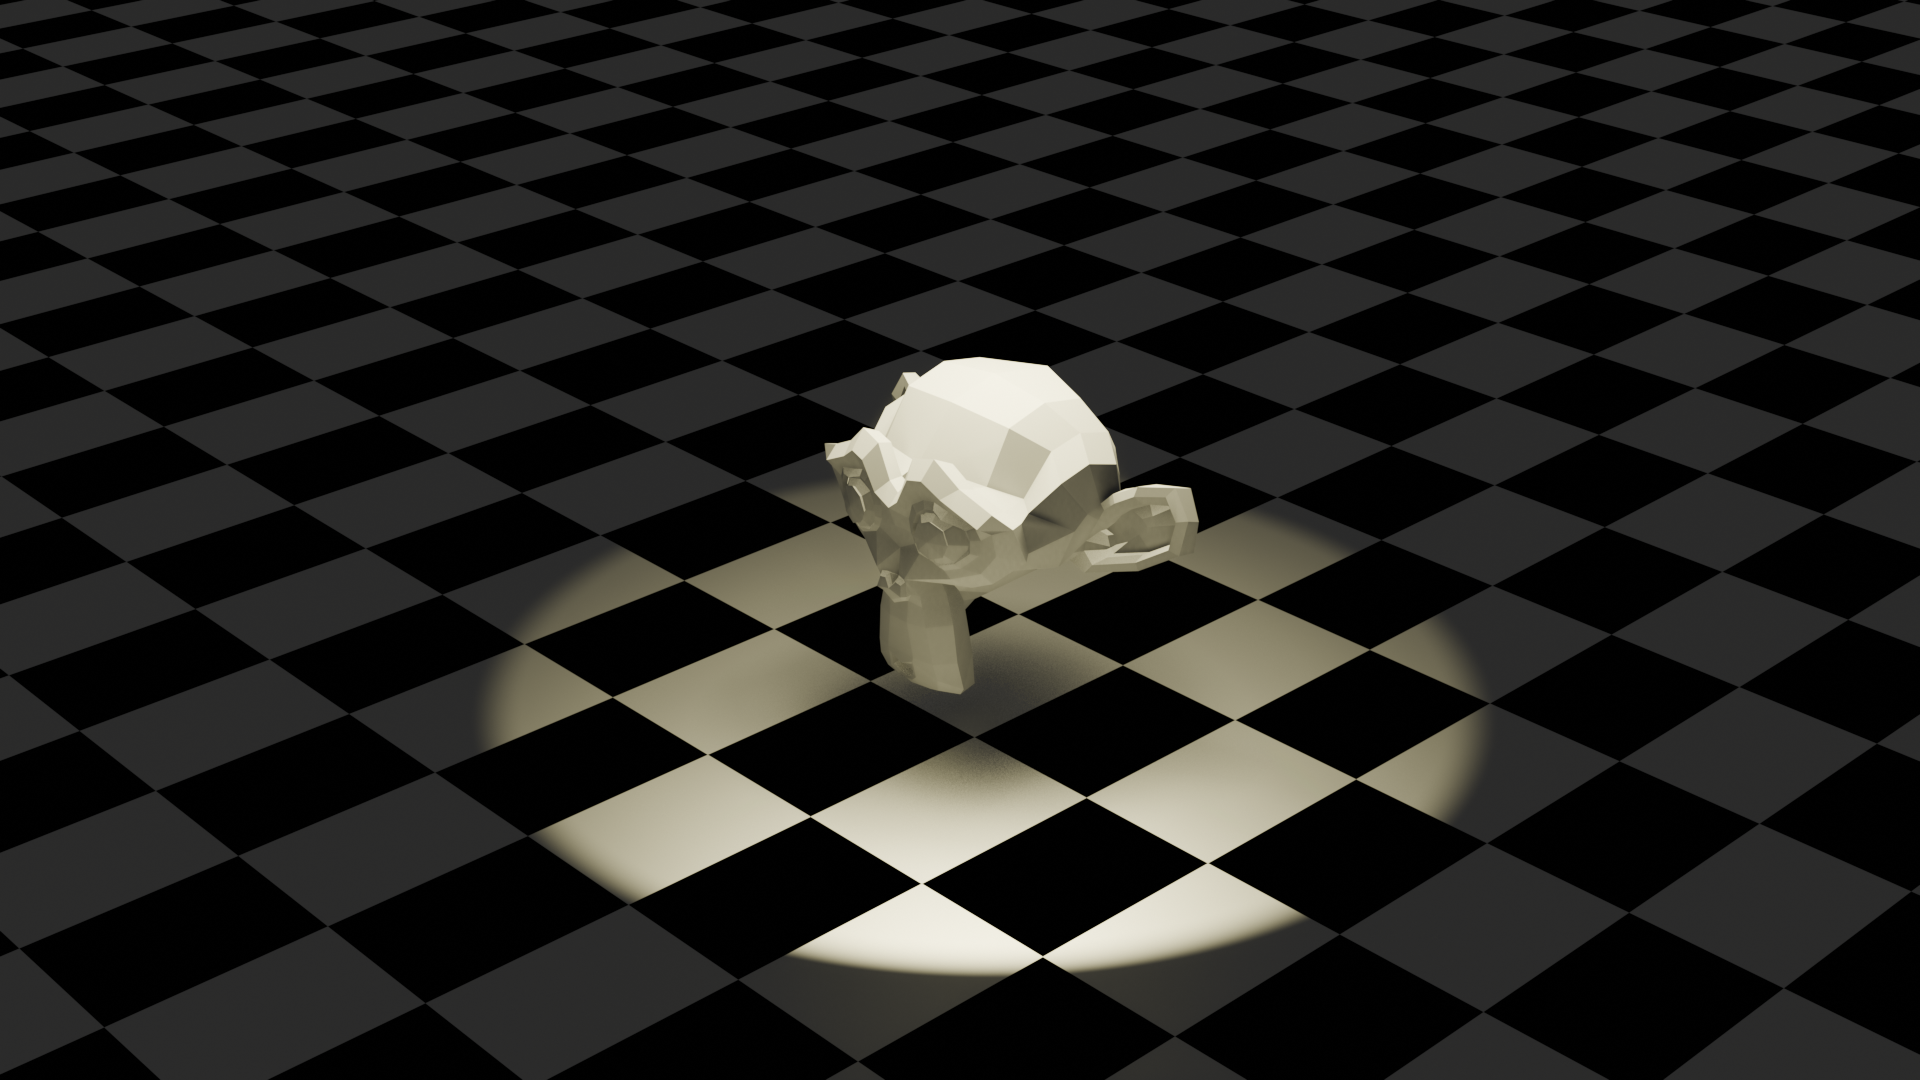
\includegraphics[width=\linewidth]{images/diffuse.png}
          \caption*{Low specular}
        \end{figure}
        \begin{figure}
          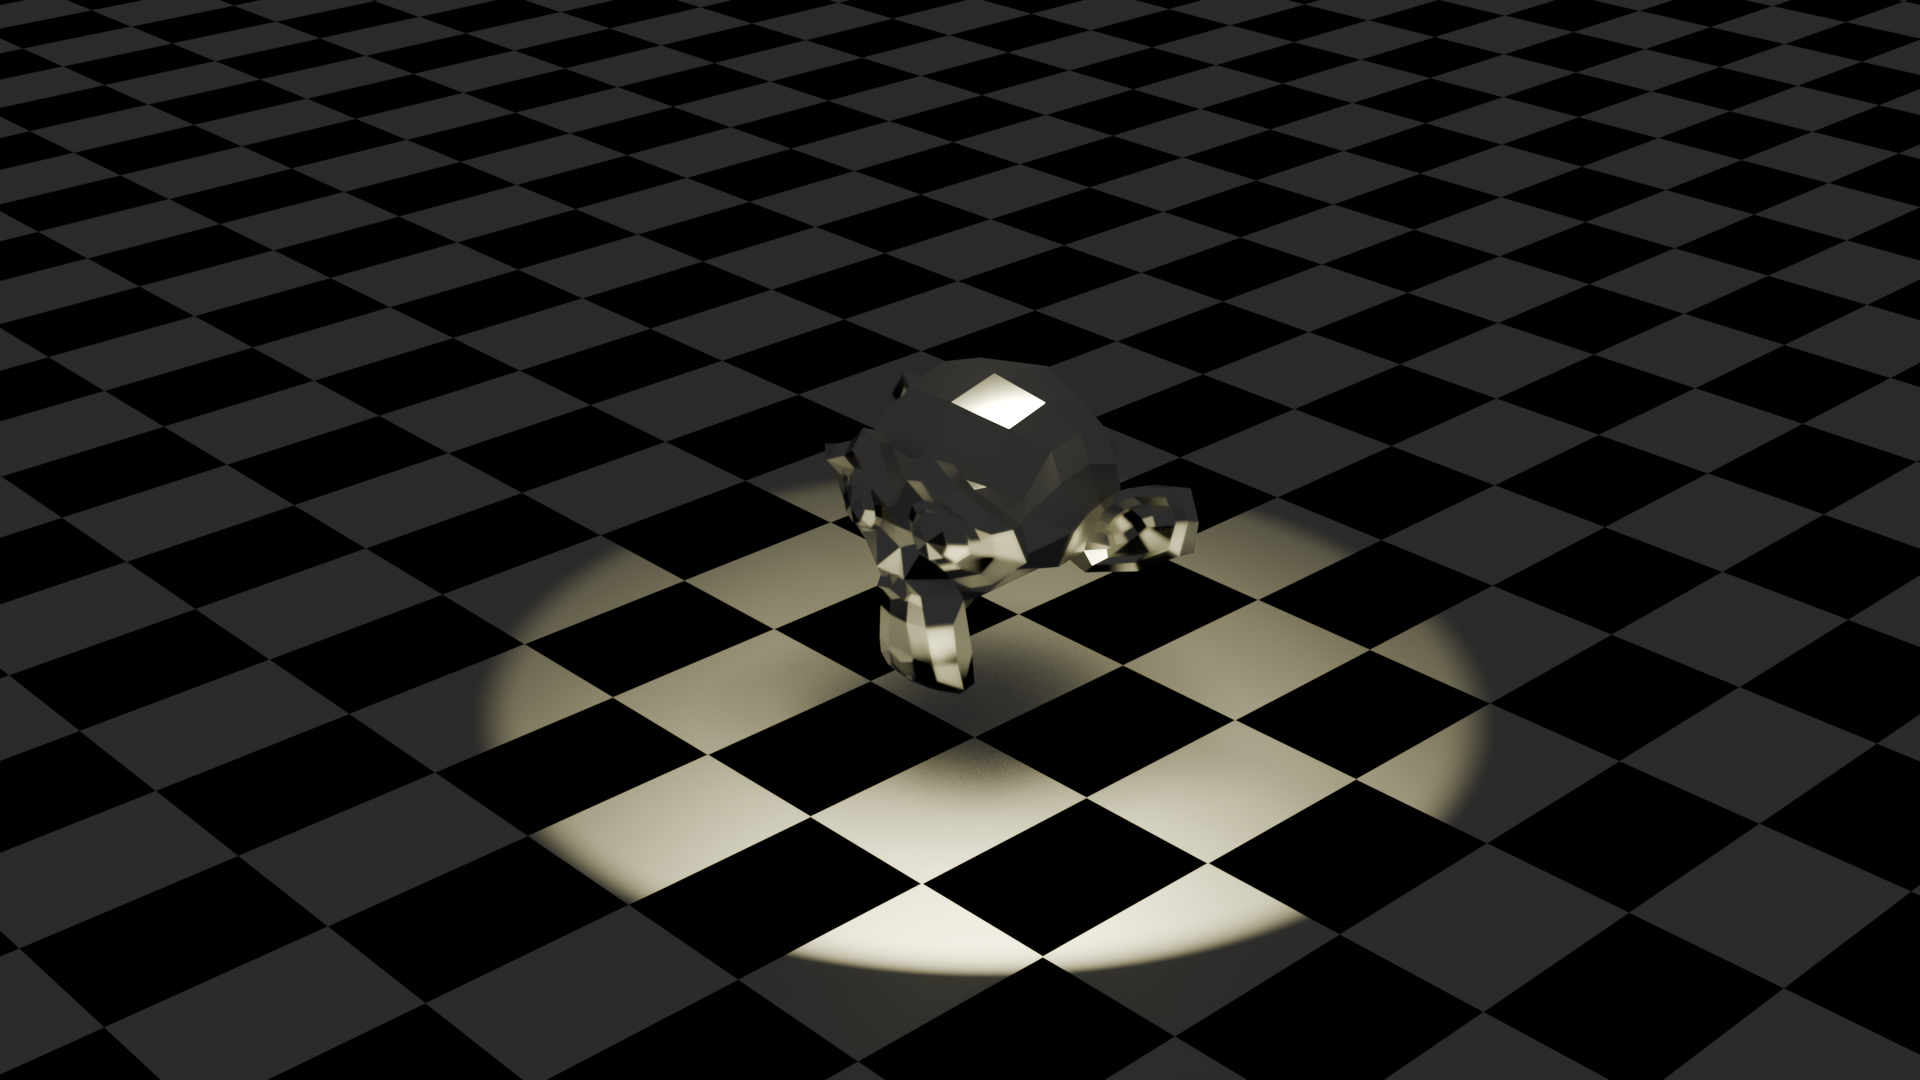
\includegraphics[width=\linewidth]{images/specular.png}
          \caption*{High specular}
        \end{figure}
      }
    \end{column}
  \end{columns}
\end{frame}

\begin{frame}{Shininess Parameter (n) - Effect on Highlights}
  \begin{columns}
    \begin{column}{0.5\textwidth}
      \begin{mathbox}{Shininess Exponent}
        \small
        \textbf{Mathematical effect:}
        \begin{align*}
          (\cos(\alpha))^n
        \end{align*}

        \textbf{As $n$ increases:}
        \begin{itemize}
          \item Highlight becomes smaller
          \item Highlight becomes sharper
          \item Material appears shinier
        \end{itemize}
      \end{mathbox}
    \end{column}
    \begin{column}{0.5\textwidth}
      \begin{figure}
        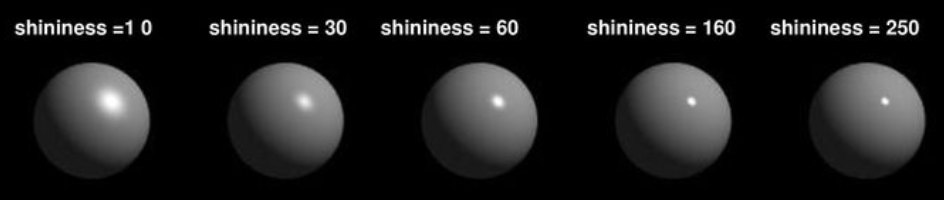
\includegraphics[width=\linewidth]{images/shininess.png}
        \caption*{\scriptsize Spheres with different shininess parameters}
      \end{figure}
      \vspace{0.3cm}
      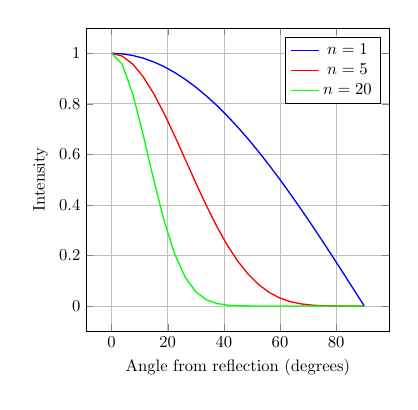
\begin{tikzpicture}[scale=0.6]
        % Plot of cosine functions with different powers
        \begin{axis}[
            width=8cm,
            height=8cm,
            domain=0:90,
            xlabel={Angle from reflection (degrees)},
            ylabel={Intensity},
            legend pos=north east,
            grid=major
          ]
          \addplot[blue, thick] {(cos(x))^1};
          \addlegendentry{$n=1$}
          \addplot[red, thick] {(cos(x))^5};
          \addlegendentry{$n=5$}
          \addplot[green, thick] {(cos(x))^20};
          \addlegendentry{$n=20$}
        \end{axis}
      \end{tikzpicture}
    \end{column}
  \end{columns}
\end{frame}

\begin{frame}{Complete Phong Equation Assembly}
  \begin{mathbox}{Putting It All Together}
    \textbf{Complete Phong illumination model:}
    \begin{align*}
      I &= I_{\text{ambient}} + I_{\text{diffuse}} + I_{\text{specular}}
    \end{align*}

    \pause
    \begin{align*}
      \mathbf{I} &= \mathbf{k}_a \odot \mathbf{I_a} + \sum_{i=1}^{n} \mathbf{I_{l_i}} \odot \left[ \mathbf{k}_d \max(0, \mathbf{N} \cdot \mathbf{L}_i) + \mathbf{k}_s \max(0, \mathbf{R}_i \cdot \mathbf{V})^n \right]
    \end{align*}
  \end{mathbox}
\end{frame}
